\section{DVND} \label{sec:res_df_dvnd}

Uma solução inicial aleatória é enviada para os processos de busca DVND e RVND, então o valor médio da função objetivo é apresentado nas Tabelas~\ref{tab:rvndDvndN1imp},~\ref{tab:rvndDvndN2imp},~\ref{tab:rvndDvndN3imp} e~\ref{tab:rvndDvndN4imp}.
Este resultado foi obtido de um conjunto de 100 execuções, foram comparadas a versão do RVND em dataflow com o DVND em dataflow, sendo este último sujeito a seguinte parametrização: número de máquinas usadas $m \in [1, 4]$ e número de processos por máquina $w \in [1, 10]$.
O valor expresso é o fator de melhoria sobre a solução inicial $Imp$ que é definido por $\frac{Inicial}{Final}$, onde $Inicial$ é o valor para a função objetivo da solução inicial, a magnitude de \textit{Imp} indica a melhora obtida na solução por cada método respectivamente.

\begin{table}[htbp]
\caption{Comparação dos resultados de melhoria no valor da solução para uma máquina variando a quantidade de processos $w$}
\begin{center}
\begin{tabular}{cccccccccccc}
\hline
\hline
\multicolumn{2}{c}{} &\multicolumn{10}{c}{\textbf{DVND $m=1$}} \\
\cline{3-12}
\textbf{\#} & \textbf{RVND}& \textbf{w1}& \textbf{w2}& \textbf{w3}& \textbf{w4}& \textbf{w5}& \textbf{w6}& \textbf{w7}& \textbf{w8}& \textbf{w9}& \textbf{w10} \\
\hline
0 & 3,83& 3,85& 3,83& 3,82& 3,82& \textbf{3,87}& 3,85& 3,85& \textbf{3,87}& 3,76& 3,85 \\
1 & 8,35& \textbf{8,51}& 8,40& 8,45& 8,48& 8,43& 8,46& 8,48& 8,49& 8,49& 8,47 \\
2 & 1,71& \textbf{1,87}& \textbf{1,87}& \textbf{1,87}& \textbf{1,87}& \textbf{1,87}& \textbf{1,87}& 1,86& \textbf{1,87}& 1,85& 1,85 \\
2 & 2,71& 2,65& 2,71& \textbf{2,74}& \textbf{2,74}& 2,73& \textbf{2,74}& 2,71& 2,71& 2,70& 2,72 \\
4 &\textbf{16,83}&16,43&16,58&16,64&16,65&16,65&16,66&16,66&16,69&16,70&16,69 \\
5 & 5,50& \textbf{5,65}& 5,49& 5,54& 5,54& 5,52& 5,54& 5,51& 5,55& 5,52& 5,49 \\
6 & 8,30& 8,29& 8,34& 8,34& 8,34& 8,34& 8,35& 8,34& 8,33& 8,34& \textbf{8,36} \\
7 &24,14&23,93&24,09&24,08&24,13&24,09&24,09&24,08&24,11&24,09& \textbf{24,16} \\
\hline
\end{tabular}
\label{tab:rvndDvndN1imp}
\end{center}
\end{table}

\begin{table}[htbp]
\caption{Comparação dos resultados de melhoria no valor da solução para duas máquinas variando a quantidade de processos $w$}
\begin{center}
\begin{tabular}{cccccccccccc}
\hline
\hline
\multicolumn{2}{c}{} &\multicolumn{10}{c}{\textbf{DVND $m=2$}} \\
\cline{3-12}
\textbf{\#} & \textbf{RVND}& \textbf{w1}& \textbf{w2}& \textbf{w3}& \textbf{w4}& \textbf{w5}& \textbf{w6}& \textbf{w7}& \textbf{w8}& \textbf{w9}& \textbf{w10} \\
\hline
0 & 3,83& 3,82& 3,90& \textbf{3,95}& 3,91& 3,86& 3,90& 3,87& 3,87& 3,88& 3,90 \\
1 & 8,35& 8,54& \textbf{8,57}& 8,53& 8,52& 8,56& 8,52& 8,52& 8,51& 8,49& \textbf{8,57} \\
2 & 1,71& \textbf{1,87}& \textbf{1,87}& \textbf{1,87}& \textbf{1,87}& 1,85& 1,86& 1,85& 1,84& 1,85& 1,86 \\
3 & 2,71& 2,76& \textbf{2,79}& 2,74& 2,75& 2,74& 2,67& 2,70& 2,70& 2,72& 2,71 \\
4 &\textbf{16,83}&16,63&16,64&16,66&16,67&16,72&16,66&16,68&16,68&16,67&16,67 \\
5 & 5,50& \textbf{5,57}& 5,54& 5,50& 5,51& 5,50& 5,50& 5,48& 5,51& 5,51& 5,51 \\
6 & 8,30& 8,36& 8,33& 8,35& 8,35& 8,35& \textbf{8,36}& 8,32& 8,31& 8,33& 8,35 \\
7 &\textbf{24,14}&23,97&24,04&24,08&24,05&24,08&24,12&24,10&24,12&24,15&\textbf{24,14} \\
\hline
\end{tabular}
\label{tab:rvndDvndN2imp}
\end{center}
\end{table}

\begin{table}[htbp]
\caption{Comparação dos resultados de melhoria no valor da solução para três máquinas variando a quantidade de processos $w$}
\begin{center}
\begin{tabular}{cccccccccccc}
\hline
\hline
\multicolumn{2}{c}{} &\multicolumn{10}{c}{\textbf{DVND $m=3$}} \\
\cline{3-12}
\textbf{\#} & \textbf{RVND}& \textbf{w1}& \textbf{w2}& \textbf{w3}& \textbf{w4}& \textbf{w5}& \textbf{w6}& \textbf{w7}& \textbf{w8}& \textbf{w9}& \textbf{w10} \\
\hline
0 & 3,83& 3,93& \textbf{3,94}& 3,90& 3,94& 3,92& 3,90& 3,88& 3,91& 3,93& 3,86 \\
1 & 8,35& \textbf{8,60}& 8,56& 8,49& 8,53& 8,59& 8,53& 8,49& 8,49& 8,52& 8,53 \\
2 & 1,71& \textbf{1,87}& \textbf{1,87}& 1,85& 1,86& 1,86& 1,84& 1,86& 1,86& 1,87& 1,86 \\
3 & 2,71& 2,68& 2,70& \textbf{2,72}& 2,70& 2,71& \textbf{2,72}& 2,69& 2,71& 2,70& 2,69 \\
4 &\textbf{16,83}&16,63&16,68&16,72&16,68&16,70&16,67&16,72&16,71&16,72&16,72 \\
5 & 5,50& \textbf{5,55}& 5,52& 5,48& 5,52& 5,53& 5,51& 5,49& 5,50& 5,53& 5,49 \\
6 & 8,30& \textbf{8,35}& 8,33& 8,29& \textbf{8,35}& \textbf{8,35}& \textbf{8,35}& 8,33& \textbf{8,35}& 8,33& 8,32 \\
7 &\textbf{24,14}&23,95&24,06&\textbf{24,14}&24,09&\textbf{24,14}&24,10&24,09&24,10&\textbf{24,14}&24,10 \\
\hline
\end{tabular}
\label{tab:rvndDvndN3imp}
\end{center}
\end{table}

\begin{table}[htbp]
\caption{Comparação dos resultados de melhoria no valor da solução para quatro máquinas variando a quantidade de processos $w$}
\begin{center}
\begin{tabular}{cccccccccccc}
\hline
\hline
\multicolumn{2}{c}{} &\multicolumn{10}{c}{\textbf{DVND $m=4$}} \\
\cline{3-12}
\textbf{\#} & \textbf{RVND}& \textbf{w1}& \textbf{w2}& \textbf{w3}& \textbf{w4}& \textbf{w5}& \textbf{w6}& \textbf{w7}& \textbf{w8}& \textbf{w9}& \textbf{w10} \\
\hline
0 & 3,83& \textbf{3,94}& 3,93& 3,89& 3,89& 3,92& 3,93& 3,89& \textbf{3,94}& 3,92& \textbf{3,94} \\
1 & 8,35& \textbf{8,57}& \textbf{8,57}& 8,52& 8,49& \textbf{8,57}& 8,55& 8,50& 8,53& 8,53& 8,56 \\
2 & 1,71& \textbf{1,87}& \textbf{1,87}& 1,86& 1,84& 1,86& 1,86& \textbf{1,87}& 1,85& \textbf{1,87}& \textbf{1,87} \\
3 & 2,71& 2,68& 2,71& 2,69& 2,70& 2,69& \textbf{2,73}& 2,67& 2,70& 2,70& 2,69 \\
4 &\textbf{16,83}&16,66&16,70&16,68&16,70&16,69&16,71&16,67&16,66&16,70&16,68 \\
5 & 5,50& \textbf{5,55}& \textbf{5,55}& 5,51& 5,47& 5,54& 5,49& 5,50& 5,50& 5,54& 5,51 \\
6 & 8,30& 8,34& 8,33& 8,34& 8,33& 8,34& 8,34& \textbf{8,35}& 8,33& 8,34& 8,33 \\
7 &24,14&24,01&\textbf{24,15}&24,10&24,10&24,11&24,11&24,13&24,14&24,13&24,11 \\
\hline
\end{tabular}
\label{tab:rvndDvndN4imp}
\end{center}
\end{table}

De forma equivalente, as Tabelas~\ref{tab:rvndDvndN1times},~\ref{tab:rvndDvndN2times},~\ref{tab:rvndDvndN3times} e~\ref{tab:rvndDvndN4times} indicam o tempo médio de execução para o RVND e DVND (em segundos).
As colunas indicam os valores de tempo para as variações do método DVND conforme mencionado anteriormente.
Da tabela podemos ver que, para as instâncias 0 a 4 ($n \in \{52, 100, 226, 318\}$), o DVND consume um tempo computacional maior que o RVND mesmo utilizando mais máquinas e processos, contudo a partir da instancia 4 ($n=501$) o DVND supera os tempos alcançados pelo RVND, variando apenas sua qualidade conforme os parâmetros de número de máquinas ($m$) e processos($w$), o que comprova a tese levantada em~\cite{df-dvnd2018} de que melhorias na implementação poderiam alterar significativamente o desempenho do método.
%, being more expensive in all instances proportionally to the number of parallel neighborhood exploration calls (slightly more than five, as explained in subsection \ref{subsec:neighborhoods}).

Cabe ressaltar que o desempenho de uma configuração com duas máquinas ($m=2$) e dois processos ($w=2$) não é equivalente ao de uma máquina ($m=1$) e quatro processos ($w=4$), nos dois casos são 4 processos contudo no primeiro estes rodam em máquinas diferentes e se comunicam via troca de mensagens pela rede enquanto na segunda rodam na mesma máquina.
No primeiro caso estão sujeitos ao ambiente distribuído enquanto no segundo caso apesar de rodar na mesma máquina usa apenas uma placa de vídeo logo há uma concorrência pelo uso dos recursos.

\begin{table}[htbp]
\caption{Comparação dos resultados de tempo para uma máquina variando a quantidade de processos $w$}
\begin{center}
\begin{tabular}{cccccccccccc}
\hline
\hline
\multicolumn{2}{c}{} &\multicolumn{10}{c}{\textbf{DVND $m=1$}} \\
\cline{3-12}
\textbf{\#} & \textbf{RVND}& \textbf{w1}& \textbf{w2}& \textbf{w3}& \textbf{w4}& \textbf{w5}& \textbf{w6}& \textbf{w7}& \textbf{w8}& \textbf{w9}& \textbf{w10} \\
\hline
0 & \textbf{1,08}& 1,25& 1,25& 1,30&1,36&1,43&1,49&1,58&1,65&1,73&1,81 \\
1 & \textbf{1,18}& 1,47& 1,35& 1,41&1,47&1,53&1,58&1,65&1,73&1,82&1,88 \\
2 & \textbf{1,25}& 1,34& 1,28& 1,33&1,40&1,47&1,53&1,63&1,68&1,80&1,87 \\
3 & \textbf{1,74}& 2,46& 1,92& 1,81&1,78&1,80&1,87&1,93&2,00&2,08&2,13 \\
4 & 4,30& 3,96& 3,19& 2,88&2,71&\textbf{2,66}&2,74&2,78&2,88&3,03&3,10 \\
5 & 4,94& 6,31& 4,19& 3,47&3,21&\textbf{3,03}&3,11&3,13&3,23&3,31&3,31 \\
6 & 7,58& 9,20& 6,01& 4,78&4,41&\textbf{4,05}&4,07&4,18&4,23&4,26&4,34 \\
7 & 25,43&22,43&14,74&11,26&9,43&8,56&\textbf{8,50}&8,65&8,90&8,93&9,03 \\
\hline
\end{tabular}
\label{tab:rvndDvndN1times}
\end{center}
\end{table}

\begin{table}[htbp]
\caption{Comparação dos resultados de tempo para duas máquinas variando a quantidade de processos $w$}
\begin{center}
\begin{tabular}{cccccccccccc}
\hline
\hline
\multicolumn{2}{c}{} &\multicolumn{10}{c}{\textbf{DVND $m=2$}} \\
\cline{3-12}
\textbf{\#} & \textbf{RVND}& \textbf{w1}& \textbf{w2}& \textbf{w3}& \textbf{w4}& \textbf{w5}& \textbf{w6}& \textbf{w7}& \textbf{w8}& \textbf{w9}& \textbf{w10} \\
\hline
0 & \textbf{1,08}& 1,24&1,26&1,31&1,43&2,53&2,66&2,59&2,70&2,62&2,58 \\
1 & \textbf{1,18}& 1,46&1,42&1,47&1,60&2,63&2,72&2,66&2,70&2,86&2,66 \\
2 & \textbf{1,25}& 1,30&1,30&1,38&1,46&2,66&2,71&2,70&2,78&2,79&2,71 \\
3 & \textbf{1,74}& 2,20&1,79&1,75&1,87&2,95&2,96&2,93&3,00&3,01&2,94 \\
4 & 4,30& 4,14&2,93&\textbf{2,72}&\textbf{2,72}&3,55&3,73&3,77&3,70&3,93&3,84 \\
5 & 4,94& 4,93&3,39&\textbf{2,83}&2,86&3,72&3,82&3,76&3,75&4,07&3,97 \\
6 & 7,58& 6,48&4,48&\textbf{3,69}&3,76&4,34&4,59&4,43&4,40&4,71&4,77 \\
7 & 25,43&14,68&9,03&7,57&\textbf{7,43}&8,43&8,25&8,85&8,74&8,76&8,89 \\
\hline
\end{tabular}
\label{tab:rvndDvndN2times}
\end{center}
\end{table}

\begin{table}[htbp]
\caption{Comparação dos resultados de tempo para três máquinas variando a quantidade de processos $w$}
\begin{center}
\begin{tabular}{cccccccccccc}
\hline
\hline
\multicolumn{2}{c}{} &\multicolumn{10}{c}{\textbf{DVND $m=3$}} \\
\cline{3-12}
\textbf{\#} & \textbf{RVND}& \textbf{w1}& \textbf{w2}& \textbf{w3}& \textbf{w4}& \textbf{w5}& \textbf{w6}& \textbf{w7}& \textbf{w8}& \textbf{w9}& \textbf{w10} \\
\hline
0 & \textbf{1,08}& 1,21&1,26&2,30&2,36&2,56&2,67&2,72&2,94&2,98&2,93 \\
1 & \textbf{1,18}& 1,36&1,42&2,28&2,40&2,64&2,75&2,91&3,05&3,06&3,02 \\
2 & \textbf{1,25}& 1,29&1,30&2,37&2,45&2,59&2,78&2,85&2,97&3,01&3,07 \\
3 & \textbf{1,74}& 1,92&1,84&2,56&2,78&2,93&3,04&3,13&3,25&3,33&3,28 \\
4 & 4,30& 3,39&\textbf{3,05}&3,50&3,77&4,07&4,23&4,43&4,54&4,63&4,66 \\
5 & 4,94& 3,99&\textbf{3,17}&3,28&3,88&4,11&4,21&4,36&4,43&4,65&4,52 \\
6 & 7,58& 5,26&3,99&\textbf{3,88}&4,58&4,76&4,94&4,96&5,07&5,35&5,22 \\
7 &25,43&10,66&\textbf{7,32}&8,04&8,11&8,70&8,96&9,01&9,11&9,35&9,33 \\
\hline
\end{tabular}
\label{tab:rvndDvndN3times}
\end{center}
\end{table}

\begin{table}[htbp]
\caption{Comparação dos resultados de tempo para quatro máquinas variando a quantidade de processos $w$}
\begin{center}
\begin{tabular}{cccccccccccc}
\hline
\hline
\multicolumn{2}{c}{} &\multicolumn{10}{c}{\textbf{DVND $m=4$}} \\
\cline{3-12}
\textbf{\#} & \textbf{RVND}& \textbf{w1}& \textbf{w2}& \textbf{w3}& \textbf{w4}& \textbf{w5}& \textbf{w6}& \textbf{w7}& \textbf{w8}& \textbf{w9}& \textbf{w10} \\
\hline
0 & \textbf{1,08}&1,21&2,13&2,41&2,54&2,75&2,94&3,05&3,17&3,13&3,35 \\
1 & \textbf{1,18}&1,38&2,18&2,48&2,62&2,78&3,12&3,16&3,27&3,44&3,51 \\
2 & \textbf{1,25}&1,28&2,15&2,45&2,59&2,85&3,03&3,15&3,19&3,29&3,38 \\
3 & \textbf{1,74}&1,85&2,21&2,86&2,92&3,17&3,32&3,40&3,52&3,58&3,73 \\
4 & 4,30&\textbf{3,08}&3,23&3,92&4,11&4,39&4,49&4,63&4,64&4,68&4,87 \\
5 & 4,94&3,40&\textbf{3,17}&3,86&3,94&4,44&4,46&4,57&4,60&4,71&4,85 \\
6 & 7,58&4,36&\textbf{3,87}&4,59&4,50&5,13&4,98&5,28&5,28&5,40&5,68 \\
7 & 25,43&8,70&\textbf{7,76}&8,00&8,53&9,02&8,98&9,19&9,37&9,46&9,31 \\
\hline
\end{tabular}
\label{tab:rvndDvndN4times}
\end{center}
\end{table}

% \begin{figure}%
    \centering
    \subfloat[Instância 0]{{
        \includegraphics[scale=0.4]{figuras/dvnd/n1/time0.png}
        \label{fig:timeDvndRvnd_n1in0}
    }}%
    \qquad
    \subfloat[Instância 1]{{
        \includegraphics[scale=0.4]{figuras/dvnd/n1/time1.png}
        \label{fig:timeDvndRvnd_n1in1}
    }}%
    \caption{Tempos DVND e RVND das instâncias 0 e 1 para $n=1$.}%
    \label{fig:timeDvndRvnd_n1in0_1}%
\end{figure}

\begin{figure}%
    \centering
    \subfloat[Instância 2]{{
        \includegraphics[scale=0.4]{figuras/dvnd/n1/time2.png}
        \label{fig:timeDvndRvnd_n1in2}
    }}%
    \qquad
    \subfloat[Instância 3]{{
        \includegraphics[scale=0.4]{figuras/dvnd/n1/time3.png}
        \label{fig:timeDvndRvnd_n1in3}
    }}%
    \caption{Tempos DVND e RVND das instâncias 2 e 3 para $n=1$.}%
    \label{fig:timeDvndRvnd_n1in2_3}%
\end{figure}

\begin{figure}%
    \centering
    \subfloat[Instância 4]{{
        \includegraphics[scale=0.4]{figuras/dvnd/n1/time4.png}
        \label{fig:timeDvndRvnd_n1in4}
    }}%
    \qquad
    \subfloat[Instância 5]{{
        \includegraphics[scale=0.4]{figuras/dvnd/n1/time5.png}
        \label{fig:timeDvndRvnd_n1in5}
    }}%
    \caption{Tempos DVND e RVND das instâncias 4 e 5 para $n=1$.}%
    \label{fig:timeDvndRvnd_n1in4_5}%
\end{figure}

\begin{figure}%
    \centering
    \subfloat[Instância 6]{{
        \includegraphics[scale=0.4]{figuras/dvnd/n1/time6.png}
        \label{fig:timeDvndRvnd_n1in6}
    }}%
    \qquad
    \subfloat[Instância 7]{{
        \includegraphics[scale=0.4]{figuras/dvnd/n1/time7.png}
        \label{fig:timeDvndRvnd_n1in7}
    }}%
    \caption{Tempos DVND e RVND das instâncias 6 e 7 para $n=1$.}%
    \label{fig:timeDvndRvnd_n1in6_7}%
\end{figure}

% \begin{figure}%
    \centering
    \subfloat[Instância 0]{{
        \includegraphics[scale=0.4]{figuras/dvnd/n2/time0.png}
        \label{fig:timeDvndRvnd_n2in0}
    }}%
    \qquad
    \subfloat[Instância 1]{{
        \includegraphics[scale=0.4]{figuras/dvnd/n2/time1.png}
        \label{fig:timeDvndRvnd_n2in2}
    }}%
    \caption{Tempos DVND e RVND das instâncias 0 e 1 para $n=2$.}%
    \label{fig:timeDvndRvnd_n2in0_1}%
\end{figure}

\begin{figure}%
    \centering
    \subfloat[Instância 2]{{
        \includegraphics[scale=0.4]{figuras/dvnd/n2/time2.png}
        \label{fig:timeDvndRvnd_n2in2}
    }}%
    \qquad
    \subfloat[Instância 3]{{
        \includegraphics[scale=0.4]{figuras/dvnd/n2/time3.png}
        \label{fig:timeDvndRvnd_n2in3}
    }}%
    \caption{Tempos DVND e RVND das instâncias 2 e 3 para $n=2$.}%
    \label{fig:timeDvndRvnd_n2in2_3}%
\end{figure}

\begin{figure}%
    \centering
    \subfloat[Instância 4]{{
        \includegraphics[scale=0.4]{figuras/dvnd/n2/time4.png}
        \label{fig:timeDvndRvnd_n2in4}
    }}%
    \qquad
    \subfloat[Instância 5]{{
        \includegraphics[scale=0.4]{figuras/dvnd/n2/time5.png}
        \label{fig:timeDvndRvnd_n2in5}
    }}%
    \caption{Tempos DVND e RVND das instâncias 4 e 5 para $n=2$.}%
    \label{fig:timeDvndRvnd_n2in4_5}%
\end{figure}

\begin{figure}%
    \centering
    \subfloat[Instância 6]{{
        \includegraphics[scale=0.4]{figuras/dvnd/n2/time6.png}
        \label{fig:timeDvndRvnd_n2in6}
    }}%
    \qquad
    \subfloat[Instância 7]{{
        \includegraphics[scale=0.4]{figuras/dvnd/n2/time7.png}
        \label{fig:timeDvndRvnd_n2in7}
    }}%
    \caption{Tempos DVND e RVND das instâncias 6 e 7 para $n=2$.}%
    \label{fig:timeDvndRvnd_n2in6_7}%
\end{figure}

% \begin{figure}%
    \centering
    \subfloat[Instância 0]{{
        \includegraphics[scale=0.4]{figuras/dvnd/n3/time0.png}
        \label{fig:timeDvndRvnd_n3in0}
    }}%
    \qquad
    \subfloat[Instância 1]{{
        \includegraphics[scale=0.4]{figuras/dvnd/n3/time1.png}
        \label{fig:timeDvndRvnd_n3in3}
    }}%
    \caption{Tempos DVND e RVND das instâncias 0 e 1 para $n=3$.}%
    \label{fig:timeDvndRvnd_n3in0_1}%
\end{figure}

\begin{figure}%
    \centering
    \subfloat[Instância 2]{{
        \includegraphics[scale=0.4]{figuras/dvnd/n3/time2.png}
        \label{fig:timeDvndRvnd_n3in2}
    }}%
    \qquad
    \subfloat[Instância 3]{{
        \includegraphics[scale=0.4]{figuras/dvnd/n3/time3.png}
        \label{fig:timeDvndRvnd_n3in3}
    }}%
    \caption{Tempos DVND e RVND das instâncias 2 e 3 para $n=3$.}%
    \label{fig:timeDvndRvnd_n3in2_3}%
\end{figure}

\begin{figure}%
    \centering
    \subfloat[Instância 4]{{
        \includegraphics[scale=0.4]{figuras/dvnd/n3/time4.png}
        \label{fig:timeDvndRvnd_n3in4}
    }}%
    \qquad
    \subfloat[Instância 5]{{
        \includegraphics[scale=0.4]{figuras/dvnd/n3/time5.png}
        \label{fig:timeDvndRvnd_n3in5}
    }}%
    \caption{Tempos DVND e RVND das instâncias 4 e 5 para $n=3$.}%
    \label{fig:timeDvndRvnd_n3in4_5}%
\end{figure}

\begin{figure}%
    \centering
    \subfloat[Instância 6]{{
        \includegraphics[scale=0.4]{figuras/dvnd/n3/time6.png}
        \label{fig:timeDvndRvnd_n3in6}
    }}%
    \qquad
    \subfloat[Instância 7]{{
        \includegraphics[scale=0.4]{figuras/dvnd/n3/time7.png}
        \label{fig:timeDvndRvnd_n3in7}
    }}%
    \caption{Tempos DVND e RVND das instâncias 6 e 7 para $n=3$.}%
    \label{fig:timeDvndRvnd_n3in6_7}%
\end{figure}

% \begin{figure}%
    \centering
    \subfloat[Instância 0]{{
        \includegraphics[scale=0.4]{figuras/dvnd/n4/time0.png}
        \label{fig:timeDvndRvnd_n4in0}
    }}%
    \qquad
    \subfloat[Instância 1]{{
        \includegraphics[scale=0.4]{figuras/dvnd/n4/time1.png}
        \label{fig:timeDvndRvnd_n4in4}
    }}%
    \caption{Tempos DVND e RVND das instâncias 0 e 1 para $n=4$.}%
    \label{fig:timeDvndRvnd_n4in0_1}%
\end{figure}

\begin{figure}%
    \centering
    \subfloat[Instância 2]{{
        \includegraphics[scale=0.4]{figuras/dvnd/n4/time2.png}
        \label{fig:timeDvndRvnd_n4in2}
    }}%
    \qquad
    \subfloat[Instância 3]{{
        \includegraphics[scale=0.4]{figuras/dvnd/n4/time3.png}
        \label{fig:timeDvndRvnd_n4in3}
    }}%
    \caption{Tempos DVND e RVND das instâncias 2 e 3 para $n=4$.}%
    \label{fig:timeDvndRvnd_n4in2_3}%
\end{figure}

\begin{figure}%
    \centering
    \subfloat[Instância 4]{{
        \includegraphics[scale=0.4]{figuras/dvnd/n4/time4.png}
        \label{fig:timeDvndRvnd_n4in4}
    }}%
    \qquad
    \subfloat[Instância 5]{{
        \includegraphics[scale=0.4]{figuras/dvnd/n4/time5.png}
        \label{fig:timeDvndRvnd_n4in5}
    }}%
    \caption{Tempos DVND e RVND das instâncias 4 e 5 para $n=4$.}%
    \label{fig:timeDvndRvnd_n4in4_5}%
\end{figure}

\begin{figure}%
    \centering
    \subfloat[Instância 6]{{
        \includegraphics[scale=0.4]{figuras/dvnd/n4/time6.png}
        \label{fig:timeDvndRvnd_n4in6}
    }}%
    \qquad
    \subfloat[Instância 7]{{
        \includegraphics[scale=0.4]{figuras/dvnd/n4/time7.png}
        \label{fig:timeDvndRvnd_n4in7}
    }}%
    \caption{Tempos DVND e RVND das instâncias 6 e 7 para $n=4$.}%
    \label{fig:timeDvndRvnd_n4in6_7}%
\end{figure}

\newcommand{\figureTimeDvndRvndSubFig}[2]{
    \subfloat[$m=#1$]{{ %scale=0.225
        \includegraphics[scale=0.425]{figuras/dvnd/n#1/time#2.png}
        \label{fig:timeDvndRvnd_n#1in#2}
    }}%
}

\newcommand{\figureTimeDvndRvnd}[2]{
\begin{figure}%
    \centering
    \figureTimeDvndRvndSubFig{1}{#1}
    \figureTimeDvndRvndSubFig{2}{#1}
    \qquad
    \figureTimeDvndRvndSubFig{3}{#1}
    \figureTimeDvndRvndSubFig{4}{#1}

    \caption{Tempos DVND e RVND para a instância #1, $n=#2$}%
    \label{fig:timeDvndRvnd_in#1}%
\end{figure}
}

% \figureTimeDvndRvnd{0}
% \figureTimeDvndRvnd{1}
% \figureTimeDvndRvnd{2}
% \figureTimeDvndRvnd{3}
% \figureTimeDvndRvnd{4}
% \figureTimeDvndRvnd{5}
% \figureTimeDvndRvnd{6}
% \figureTimeDvndRvnd{7}


% \begin{landscape}
\figureTimeDvndRvnd{0}{52}

Não obstante, analisar apenas o valor médio da solução e tempo gasto no processo podem levar a conclusões precipitadas, é possível, por exemplo, que uma grande amplitude nos resultados pode estar ofuscando a real qualidade do método. Assim sendo os resultados para as 100 execuções de cada instância foram apresentados num gráfico boxplot que pode ser visto nas Figuras~\ref{fig:timeDvndRvnd_n1in0}-\ref{fig:timeDvndRvnd_n4in7}, cada uma das figuras apresenta a variação de máquinas $m$ e processos para cada uma das instâncias.

\figureTimeDvndRvnd{1}{100}

Podemos ver pela Figura~\ref{fig:timeDvndRvnd_in1} que aumentar o número de processos ($w$) não melhora o tempo de execução, havendo uma melhoria bem sutil ao aumentar o número de máquinas ($m$) utilizadas contudo em todos os casos o RVND se mostrou mais eficiente.

É esperado que o RVND detenha tempos melhores para as instâncias menores devido a não necessitar realizar operações complexas e custosas, em termos computacionais, como a troca de contexto CPU-GPU e troca de mensagens em rede para comunicação dos processos.

\figureTimeDvndRvnd{2}{226}

Para o caso da instância 2 (com $n=226$), exibido na Figura~\ref{fig:timeDvndRvnd_in1}, começamos a verificar, visualmente, uma melhora bem tênue ao passar de uma para duas e três máquinas (ver Figuras~\ref{fig:timeDvndRvnd_n1in2}, \ref{fig:timeDvndRvnd_n2in2} e \ref{fig:timeDvndRvnd_n3in2}.

\figureTimeDvndRvnd{3}{318}

A Figura~\ref{fig:timeDvndRvnd_in3} representa os resultados para a instância 3 ($n=318$) vemos o tempo do DVND bem mais próximo ao do RVND.

Corroborando os resultados destacados a respeito das Tabelas~\ref{tab:rvndDvndN1times}-\ref{tab:rvndDvndN4times} podemos ver que o RVND apresenta melhores tempos para as instâncias até o tamanho de 318 nós (instância 3).
Contudo ao observamos as Figura~\ref{fig:timeDvndRvnd_in4} vemos que o resultado se altera e o DVND passa a obter melhores tempos.
De fato vemos na Figura~\ref{fig:timeDvndRvnd_n1in4} que o DVND supera o RVND para w $\in [2,10]$ e $m=1$ quando, para os demais valores de $m$ o DVND consegue melhores tempos mas não em todos os casos.
Da Figura~\ref{fig:timeDvndRvnd_in5} em diante pode-se perceber que a amplitude de tempos encontrados pelo RVND supera muito a do DVND mostrando o impacto do seu fator de aleatoriedade na eficiência do método em encontrar as melhores soluções.

\figureTimeDvndRvnd{4}{501}

Ao analisarmos a Figura~\ref{fig:timeDvndRvnd_in4} ($n=501$) vemos que o DVND começa a apresentar tempo melhor que o RVND, principalmente para a Figura~\ref{fig:timeDvndRvnd_n1in3} ($m=1$ e boa parte de Figura~\ref{fig:timeDvndRvnd_n2in3} que representa variação do método com a configuração de duas máquinas.

\figureTimeDvndRvnd{5}{657}

Pela execução da instância 5, Figura~\ref{fig:timeDvndRvnd_in5}, percebe-se um aumento significativo na amplitude dos tempos do RVND, podemos ver também que o tempo do DVND é razoavelmente menor que os tempos do RVND, destaque para a Figura~\ref{fig:timeDvndRvnd_n1in5} ($m=1$).
Para comparar os resultados do DVND com o RVND para a instância 5 do problema é preciso usar um teste não paramétrico pois para muitos dos casos não houveram evidências para afirmar que os dados seguem uma distribuição normal, o teste de Shapiro para o DVND com $m=1$ e $w=3$ com p-valor=0,700643 é um exemplo.

\figureTimeDvndRvnd{6}{783}

A medida que o tamanho das soluções aumenta, melhora também o desempenho do DVND comparado ao RVND, como é o caso da instância 6 na Figura~\ref{fig:timeDvndRvnd_in6}, onde os tempos do RVND são razoavelmente superiores.

\figureTimeDvndRvnd{7}{1001}

Os gráficos da instância 7 (Figura~\ref{fig:timeDvndRvnd_in7} ilustram bem a melhoria nos tempos do DVND em relação ao RVND para todos os valores de $m$ e $w$.
% \end{landscape}

Conforme podemos ver pelos p-valores encontrados ao testar o tempo do RVND e DVND pelo teste de nas Tabela~\ref{tab:wilcoxRvalues_w1_10}, exceto para alguns casos, destacados em negrito, existem evidências para afirmar que há diferença significativa nas amostras de tempos do RVND e DVND para as configurações testadas, fortalecendo assim a análise levantada a respeito dos gráficos apresentados.

\begin{landscape}
    \begin{table}[htbp]
    \caption{p-valores para o teste U de Mann-Whitney-Wilcoxon entre os tempos do DVND e RVND com $w \in [1, 10]$}
    \begin{center}
    \scalebox{0.81}{
        \begin{tabular}{cccccccccccc}
            \hline
            \hline
            & & \multicolumn{10}{c}{\textbf{$w$}} \\
            \cline{3-12}
            \textbf{\#} & \textbf{$m$} & \textbf{1} & \textbf{2} & \textbf{3} & \textbf{4} & \textbf{5} & \textbf{6} & \textbf{7} & \textbf{8} & \textbf{9} & \textbf{10} \\
            \hline
            \multirow{4}{*}{0} & 1 & 2.8e-34 & 2.56e-34 & 2.56e-34 & 2.56e-34 & 2.56e-34 & 2.56e-34 & 2.56e-34 & 2.56e-34 & 2.56e-34 & 2.56e-34 \\
             & 2 & 2.56e-34 & 2.56e-34 & 2.56e-34 & 2.56e-34 & 2.56e-34 & 2.56e-34 & 2.56e-34 & 2.56e-34 & 2.56e-34 & 2.56e-34 \\
             & 3 & 1.01e-33 & 4.4e-34 & 2.56e-34 & 2.56e-34 & 2.56e-34 & 2.56e-34 & 2.56e-34 & 2.56e-34 & 2.56e-34 & 2.56e-34 \\
             & 4 & 1.73e-33 & 2.56e-34 & 2.56e-34 & 2.56e-34 & 2.56e-34 & 2.56e-34 & 2.56e-34 & 2.56e-34 & 2.56e-34 & 2.56e-34 \\
            \hline
            \multirow{4}{*}{1} & 1 & 2.56e-34 & 2.86e-33 & 2.72e-34 & 2.56e-34 & 2.56e-34 & 2.56e-34 & 2.56e-34 & 2.56e-34 & 2.56e-34 & 2.56e-34 \\
             & 2 & 2.64e-34 & 2.8e-34 & 2.56e-34 & 2.56e-34 & 2.56e-34 & 2.56e-34 & 2.56e-34 & 2.56e-34 & 2.56e-34 & 2.56e-34 \\
             & 3 & 1.9e-31 & 3.17e-32 & 2.56e-34 & 2.56e-34 & 2.56e-34 & 2.56e-34 & 2.56e-34 & 2.56e-34 & 2.56e-34 & 2.56e-34 \\
             & 4 & 6e-32 & 2.56e-34 & 2.56e-34 & 2.56e-34 & 2.56e-34 & 2.56e-34 & 2.56e-34 & 2.56e-34 & 2.56e-34 & 2.56e-34 \\
            \hline
            \multirow{4}{*}{2} & 1 & 4.47e-10 & 5.1e-06 & 2.96e-09 & 1.97e-19 & 2.76e-31 & 3.16e-34 & 2.56e-34 & 2.56e-34 & 2.56e-34 & 2.56e-34 \\
             & 2 & 3.26e-07 & 1.1e-06 & 7.48e-15 & 2.44e-28 & 2.56e-34 & 2.56e-34 & 2.56e-34 & 2.56e-34 & 2.56e-34 & 2.56e-34 \\
             & 3 & 5.45e-05 & 4.97e-05 & 7.31e-34 & 3.78e-34 & 2.56e-34 & 2.56e-34 & 2.56e-34 & 2.56e-34 & 2.56e-34 & 2.56e-34 \\
             & 4 & 0.00338 & 7.09e-34 & 2.56e-34 & 2.56e-34 & 2.56e-34 & 2.56e-34 & 2.56e-34 & 2.56e-34 & 2.56e-34 & 2.56e-34 \\
            \hline
            \multirow{4}{*}{3} & 1 & 2.56e-34 & 3.24e-09 & 0.00295 & 0.0266 & 0.00517 & 9.48e-06 & 6.29e-10 & 1.84e-15 & 3.73e-20 & 3.53e-23 \\
             & 2 & 2.16e-27 & 0.01 & \textbf{0.0751} & 8.09e-06 & 1.36e-32 & 1.37e-33 & 2.24e-32 & 3.32e-33 & 6.54e-33 & 2.07e-33 \\
             & 3 & 5.35e-09 & 0.000108 & 3.78e-32 & 3.32e-33 & 1.25e-33 & 9.86e-33 & 6.68e-34 & 4.81e-34 & 4.27e-34 & 3.56e-34 \\
             & 4 & 2.89e-05 & 5.95e-27 & 2.8e-34 & 2.56e-34 & 2.8e-34 & 2.56e-34 & 2.56e-34 & 3.46e-34 & 2.56e-34 & 2.56e-34 \\
            \hline
            \multirow{4}{*}{4} & 1 & 0.0057 & 2.46e-26 & 2.13e-33 & 2.89e-34 & 2.89e-34 & 3.07e-34 & 2.98e-34 & 8.74e-34 & 1.13e-31 & 1.36e-29 \\
             & 2 & \textbf{0.244} & 2.47e-33 & 3.36e-34 & 2.8e-34 & 7.41e-14 & 1.88e-06 & 1.96e-05 & 1.86e-07 & \textbf{0.192} & 0.0214 \\
             & 3 & 1.84e-19 & 4.83e-30 & 3.24e-15 & 5.47e-06 & \textbf{0.524} & 0.00427 & 1.53e-06 & 3.98e-08 & 1.18e-09 & 4.49e-12 \\
             & 4 & 2.06e-29 & 6.27e-24 & 0.0266 & \textbf{0.381} & 4.04e-06 & 5.94e-08 & 5.39e-10 & 2.03e-10 & 4.9e-11 & 1.05e-13 \\
            \hline
            \multirow{4}{*}{5} & 1 & 2.08e-13 & 3.47e-05 & 6.39e-30 & 7.76e-34 & 2.98e-34 & 3.56e-34 & 2.72e-34 & 4.67e-34 & 1.37e-33 & 3.32e-33 \\
             & 2 & 0.0326 & 8.89e-31 & 2.56e-34 & 2.56e-34 & 1.75e-22 & 5.79e-16 & 3.51e-19 & 4.89e-19 & 1.02e-06 & 6.26e-11 \\
             & 3 & 2.99e-11 & 5.26e-34 & 1.67e-32 & 1.95e-14 & 2.65e-07 & 0.000147 & 0.0307 & \textbf{0.13} & \textbf{0.73} & \textbf{0.512} \\
             & 4 & 1.52e-30 & 6.68e-34 & 3.94e-15 & 1.91e-12 & \textbf{0.146} & \textbf{0.115} & \textbf{0.946} & \textbf{0.827} & \textbf{0.428} & \textbf{0.0813} \\
            \hline
            \multirow{4}{*}{6} & 1 & 1.23e-23 & 4.7e-13 & 1.04e-26 & 1.4e-29 & 1.54e-33 & 3.04e-33 & 2.74e-32 & 5.35e-32 & 1.1e-31 & 9.96e-31 \\
             & 2 & 4.11e-07 & 2.95e-29 & 2.56e-34 & 3.07e-34 & 2.6e-30 & 2.25e-28 & 1.25e-29 & 7.77e-30 & 3.99e-27 & 8.39e-27 \\
             & 3 & 8.48e-22 & 1.68e-33 & 9.27e-34 & 6.29e-28 & 9.32e-27 & 1.73e-25 & 2.74e-25 & 1.62e-24 & 3.73e-21 & 5.09e-23 \\
             & 4 & 1.48e-30 & 5.93e-34 & 1.37e-27 & 4.34e-29 & 1.14e-23 & 4.57e-25 & 1.18e-21 & 2.12e-22 & 1.01e-20 & 1.72e-17 \\
            \hline
            \multirow{4}{*}{7} & 1 & 0.00494 & 3.65e-30 & 2.56e-34 & 2.56e-34 & 2.56e-34 & 2.56e-34 & 2.56e-34 & 2.56e-34 & 2.56e-34 & 2.56e-34 \\
             & 2 & 2.26e-30 & 2.56e-34 & 2.56e-34 & 2.56e-34 & 2.56e-34 & 2.56e-34 & 2.56e-34 & 2.56e-34 & 2.56e-34 & 2.56e-34 \\
             & 3 & 2.56e-34 & 2.56e-34 & 2.56e-34 & 2.56e-34 & 2.56e-34 & 2.56e-34 & 2.56e-34 & 2.56e-34 & 2.56e-34 & 2.56e-34 \\
             & 4 & 2.56e-34 & 2.56e-34 & 2.56e-34 & 2.56e-34 & 2.56e-34 & 2.56e-34 & 2.56e-34 & 2.56e-34 & 2.56e-34 & 2.56e-34 \\
            \hline
        \end{tabular}
    }
    \label{tab:wilcoxRvalues_w1_10}
    \end{center}
    \end{table}
\end{landscape}

% \begin{table}[htbp]
% \caption{p-valores para o teste U de Mann-Whitney-Wilcoxon entre os tempos do DVND e RVND com $w \in [1, 5]$}
% \begin{center}
% \begin{tabular}{ccccccc}
% \hline
% & & \multicolumn{5}{c}{\textbf{$w$}} \\
% \cline{3-7}
% \textbf{\#} & \textbf{$m$} & \textbf{1} & \textbf{2} & \textbf{3} & \textbf{4} & \textbf{5} \\
% \hline
% \multirow{4}{*}{0} & 1 & 2,8e-34 & 2,56e-34 & 2,56e-34 & 2,56e-34 & 2,56e-34 \\
%  & 2 & 2,56e-34 & 2,56e-34 & 2,56e-34 & 2,56e-34 & 2,56e-34 \\
%  & 3 & 1,01e-33 & 4,4e-34 & 2,56e-34 & 2,56e-34 & 2,56e-34 \\
%  & 4 & 1,73e-33 & 2,56e-34 & 2,56e-34 & 2,56e-34 & 2,56e-34 \\
% \hline
% \multirow{4}{*}{1} & 1 & 2,56e-34 & 2,86e-33 & 2,72e-34 & 2,56e-34 & 2,56e-34 \\
%  & 2 & 2,64e-34 & 2,8e-34 & 2,56e-34 & 2,56e-34 & 2,56e-34 \\
%  & 3 & 1,9e-31 & 3,17e-32 & 2,56e-34 & 2,56e-34 & 2,56e-34 \\
%  & 4 & 6e-32 & 2,56e-34 & 2,56e-34 & 2,56e-34 & 2,56e-34 \\
% \hline
% \multirow{4}{*}{2} & 1 & 4,47e-10 & 5,1e-06 & 2,96e-09 & 1,97e-19 & 2,76e-31 \\
%  & 2 & 3,26e-07 & 1,1e-06 & 7,48e-15 & 2,44e-28 & 2,56e-34 \\
%  & 3 & 5,45e-05 & 4,97e-05 & 7,31e-34 & 3,78e-34 & 2,56e-34 \\
%  & 4 & 0,00338 & 7,09e-34 & 2,56e-34 & 2,56e-34 & 2,56e-34 \\
% \hline
% \multirow{4}{*}{3} & 1 & 2,56e-34 & 3,24e-09 & 0,00295 & 0,0266 & 0,00517 \\
%  & 2 & 2,16e-27 & 0,01 & \textbf{0,0751} & 8,09e-06 & 1,36e-32 \\
%  & 3 & 5,35e-09 & 0,000108 & 3,78e-32 & 3,32e-33 & 1,25e-33 \\
%  & 4 & 2,89e-05 & 5,95e-27 & 2,8e-34 & 2,56e-34 & 2,8e-34 \\
% \hline
% \multirow{4}{*}{4} & 1 & 0,0057 & 2,46e-26 & 2,13e-33 & 2,89e-34 & 2,89e-34 \\
%  & 2 & \textbf{0,244} & 2,47e-33 & 3,36e-34 & 2,8e-34 & 7,41e-14 \\
%  & 3 & 1,84e-19 & 4,83e-30 & 3,24e-15 & 5,47e-06 & \textbf{0,524} \\
%  & 4 & 2,06e-29 & 6,27e-24 & 0,0266 & \textbf{0,381} & 4,04e-06 \\
% \hline
% \multirow{4}{*}{5} & 1 & 2,08e-13 & 3,47e-05 & 6,39e-30 & 7,76e-34 & 2,98e-34 \\
%  & 2 & 0,0326 & 8,89e-31 & 2,56e-34 & 2,56e-34 & 1,75e-22 \\
%  & 3 & 2,99e-11 & 5,26e-34 & 1,67e-32 & 1,95e-14 & 2,65e-07 \\
%  & 4 & 1,52e-30 & 6,68e-34 & 3,94e-15 & 1,91e-12 & \textbf{0,146} \\
% \hline
% \multirow{4}{*}{6} & 1 & 1,23e-23 & 4,7e-13 & 1,04e-26 & 1,4e-29 & 1,54e-33 \\
%  & 2 & 4,11e-07 & 2,95e-29 & 2,56e-34 & 3,07e-34 & 2,6e-30 \\
%  & 3 & 8,48e-22 & 1,68e-33 & 9,27e-34 & 6,29e-28 & 9,32e-27 \\
%  & 4 & 1,48e-30 & 5,93e-34 & 1,37e-27 & 4,34e-29 & 1,14e-23 \\
% \hline
% \multirow{4}{*}{7} & 1 & 0,00494 & 3,65e-30 & 2,56e-34 & 2,56e-34 & 2,56e-34 \\
%  & 2 & 2,26e-30 & 2,56e-34 & 2,56e-34 & 2,56e-34 & 2,56e-34 \\
%  & 3 & 2,56e-34 & 2,56e-34 & 2,56e-34 & 2,56e-34 & 2,56e-34 \\
%  & 4 & 2,56e-34 & 2,56e-34 & 2,56e-34 & 2,56e-34 & 2,56e-34 \\
% \hline
% \end{tabular}
% \label{tab:wilcoxRvalues_w1_5}
% \end{center}
% \end{table}

% \begin{table}[htbp]
% \caption{p-valores para o teste U de Mann-Whitney-Wilcoxon entre os tempos do DVND e RVND com $w \in [6, 10]$}
% \begin{center}
% \begin{tabular}{ccccccc}
% \hline
% & & \multicolumn{5}{c}{\textbf{$w$}} \\
% \cline{3-7}
% \textbf{\#} & \textbf{$m$} & \textbf{6} & \textbf{7} & \textbf{8} & \textbf{9} & \textbf{10} \\
% \hline
% \multirow{4}{*}{0} & 1 & 2,56e-34 & 2,56e-34 & 2,56e-34 & 2,56e-34 & 2,56e-34 \\
%  & 2 & 2,56e-34 & 2,56e-34 & 2,56e-34 & 2,56e-34 & 2,56e-34 \\
%  & 3 & 2,56e-34 & 2,56e-34 & 2,56e-34 & 2,56e-34 & 2,56e-34 \\
%  & 4 & 2,56e-34 & 2,56e-34 & 2,56e-34 & 2,56e-34 & 2,56e-34 \\
% \hline
% \multirow{4}{*}{1} & 1 & 2,56e-34 & 2,56e-34 & 2,56e-34 & 2,56e-34 & 2,56e-34 \\
%  & 2 & 2,56e-34 & 2,56e-34 & 2,56e-34 & 2,56e-34 & 2,56e-34 \\
%  & 3 & 2,56e-34 & 2,56e-34 & 2,56e-34 & 2,56e-34 & 2,56e-34 \\
%  & 4 & 2,56e-34 & 2,56e-34 & 2,56e-34 & 2,56e-34 & 2,56e-34 \\
% \hline
% \multirow{4}{*}{2} & 1 & 3,16e-34 & 2,56e-34 & 2,56e-34 & 2,56e-34 & 2,56e-34 \\
%  & 2 & 2,56e-34 & 2,56e-34 & 2,56e-34 & 2,56e-34 & 2,56e-34 \\
%  & 3 & 2,56e-34 & 2,56e-34 & 2,56e-34 & 2,56e-34 & 2,56e-34 \\
%  & 4 & 2,56e-34 & 2,56e-34 & 2,56e-34 & 2,56e-34 & 2,56e-34 \\
% \hline
% \multirow{4}{*}{3} & 1 & 9,48e-06 & 6,29e-10 & 1,84e-15 & 3,73e-20 & 3,53e-23 \\
%  & 2 & 1,37e-33 & 2,24e-32 & 3,32e-33 & 6,54e-33 & 2,07e-33 \\
%  & 3 & 9,86e-33 & 6,68e-34 & 4,81e-34 & 4,27e-34 & 3,56e-34 \\
%  & 4 & 2,56e-34 & 2,56e-34 & 3,46e-34 & 2,56e-34 & 2,56e-34 \\
% \hline
% \multirow{4}{*}{4} & 1 & 3,07e-34 & 2,98e-34 & 8,74e-34 & 1,13e-31 & 1,36e-29 \\
%  & 2 & 1,88e-06 & 1,96e-05 & 1,86e-07 & \textbf{0,192} & 0,0214 \\
%  & 3 & 0,00427 & 1,53e-06 & 3,98e-08 & 1,18e-09 & 4,49e-12 \\
%  & 4 & 5,94e-08 & 5,39e-10 & 2,03e-10 & 4,9e-11 & 1,05e-13 \\
% \hline
% \multirow{4}{*}{5} & 1 & 3,56e-34 & 2,72e-34 & 4,67e-34 & 1,37e-33 & 3,32e-33 \\
%  & 2 & 5,79e-16 & 3,51e-19 & 4,89e-19 & 1,02e-06 & 6,26e-11 \\
%  & 3 & 0,000147 & 0,0307 & \textbf{0,13} & \textbf{0,73} & \textbf{0,512} \\
%  & 4 & \textbf{0,115} & \textbf{0,946} & \textbf{0,827} & \textbf{0,428} & \textbf{0,0813} \\
% \hline
% \multirow{4}{*}{6} & 1 & 3,04e-33 & 2,74e-32 & 5,35e-32 & 1,1e-31 & 9,96e-31 \\
%  & 2 & 2,25e-28 & 1,25e-29 & 7,77e-30 & 3,99e-27 & 8,39e-27 \\
%  & 3 & 1,73e-25 & 2,74e-25 & 1,62e-24 & 3,73e-21 & 5,09e-23 \\
%  & 4 & 4,57e-25 & 1,18e-21 & 2,12e-22 & 1,01e-20 & 1,72e-17 \\
% \hline
% \multirow{4}{*}{7} & 1 & 2,56e-34 & 2,56e-34 & 2,56e-34 & 2,56e-34 & 2,56e-34 \\
%  & 2 & 2,56e-34 & 2,56e-34 & 2,56e-34 & 2,56e-34 & 2,56e-34 \\
%  & 3 & 2,56e-34 & 2,56e-34 & 2,56e-34 & 2,56e-34 & 2,56e-34 \\
%  & 4 & 2,56e-34 & 2,56e-34 & 2,56e-34 & 2,56e-34 & 2,56e-34 \\
% \hline
% \end{tabular}
% \label{tab:wilcoxRvalues_w6_10}
% \end{center}
% \end{table}

Conforme podemos verificar nas Figuras~\ref{fig:timeDvndRvnd_in4}, \ref{fig:timeDvndRvnd_in5}, \ref{fig:timeDvndRvnd_in6} e \ref{fig:timeDvndRvnd_in7}, aumentar o número de processos ($mw$) no DVND melhora o tempo computacional até um ponto e então começa a degradar a performance.
Alguns possíveis motivos levantados para esse problema são a concorrência por recursos pois cada máquina utiliza apenas uma placa de vĩdeo, o que se espera implementar e avaliar, conforme descrito em propostas futuras na seção \ref{subsec:usarDuasPlacasVideo}.
Também é possível que o tamanho das instâncias avaliadas não seja suficiente para proporcionar toda a demanda de computação necessária para fazer uso dos recursos disponíveis, para avaliar essa hipótese é proposto na seção \ref{subsec:instanciasMaiores} a utilização de problemas maiores mesmo que de problemas distintos.
Outro grande fator que pode estar limitando a melhoria na performance é, conforme discutido na seção \ref{subsec:metodologiaDecomposicaoVizinhancas}, o alcance do limite de paralelização horizontal para o método, demandando assim a utilização da decomposição de vizinhnças para melhorar a capacidade de paralelismo horizontal.

Embora bastante promissor, do ponto de vista de computação paralela, é muito desafiador, no contexto da otimização, lidar com instâncias com mais de $1000$ nós, isto se deve ao fato de a busca local ser apenas uma parte da meta-heurística de busca, apresentado e publicado em~\cite{jpdc2017}, que repete o processo de busca local (RVND ou DVND) milhares de vezes.

%Another point is that, like said in Subsection~\ref{subsec:neighborhoods}, the DVND enumerates much more neighborhoods than RVND.

% O valor da solução (ótimo local encontrado) não é dominado por nenhum dos métodos, pode-se ver pela Figura~\ref{fig:valueDvndRvnd} que para alguns instâncias (1, 2 e 5) DVND obteve melhores resultados mas para as outras (3 e 4) o RVND o superou.
% Sabendo disso é importante ser feita uma maior investigação sobre o impacto destes métodos no valor da solução, a Figura~\ref{fig:valueDvndRvnd_in0} mostra que o RVND obteve melhores resultados para a maioria dos testes contudo também obteve os piores resultados para instância 0.

% \begin{figure}[htbp]
% \centerline{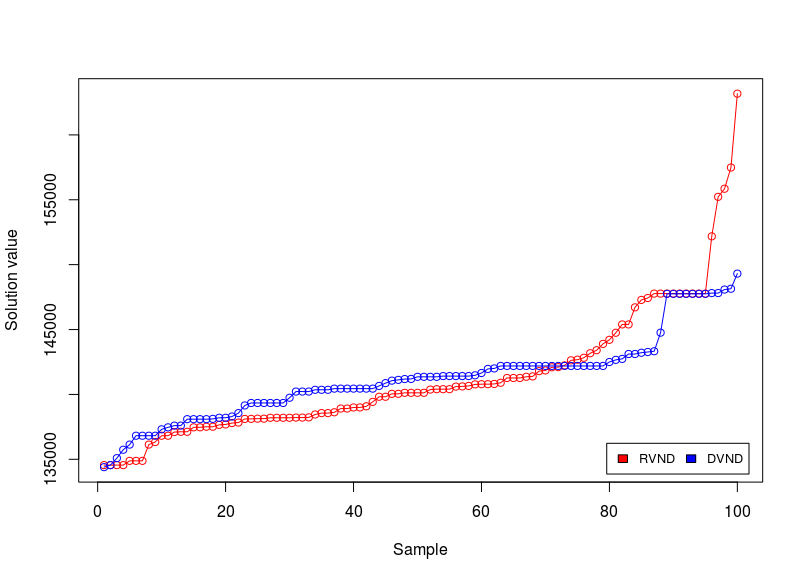
\includegraphics[scale=0.425]{figuras/dvnd/valueDvndRvnd_in0.png}}
% \caption{Valores do DVND e RVND para a instância 0}
% \label{fig:valueDvndRvnd_in0}
% \end{figure}

% Como observado na Figura~\ref{fig:valueDvndRvnd} podemos confirmar pela Figura~\ref{fig:valueDvndRvnd_in1} que o DVND obteve melhores resultados para a maior parte dos testes na instância 1.
% Um outro ponto é que o RVND obteve os piores resultados.

% \begin{figure}[htbp]
% \centerline{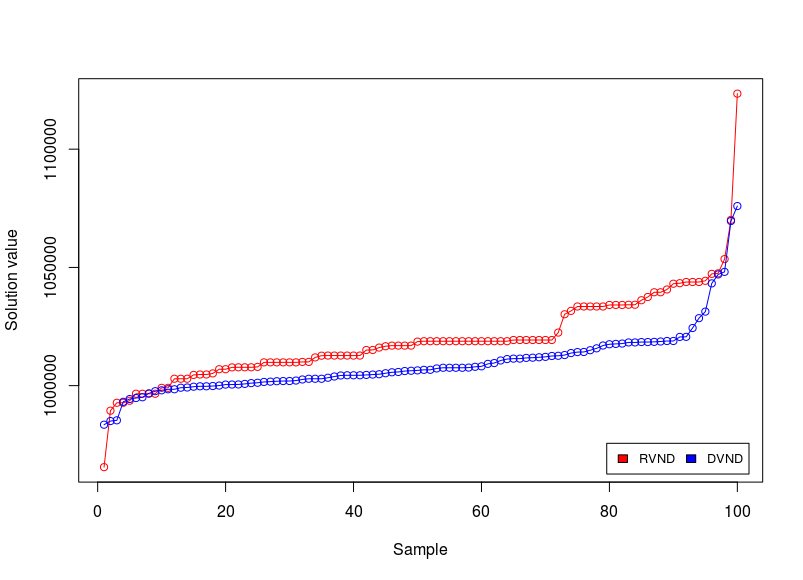
\includegraphics[scale=0.425]{figuras/dvnd/valueDvndRvnd_in1.png}}
% \caption{Valores do DVND e RVND para a instância 1}
% \label{fig:valueDvndRvnd_in1}
% \end{figure}

% A instância 2 obteve um resultado bastante diferenciado, DVND teve um comportamento muito mais regular em termos de valor da solução com uma grande discrepância em relação aos resultados encontrados pelo RVND, conforme pode ser visto na Figura~\ref{fig:valueDvndRvnd_in2}.

% \begin{figure}[htbp]
% \centerline{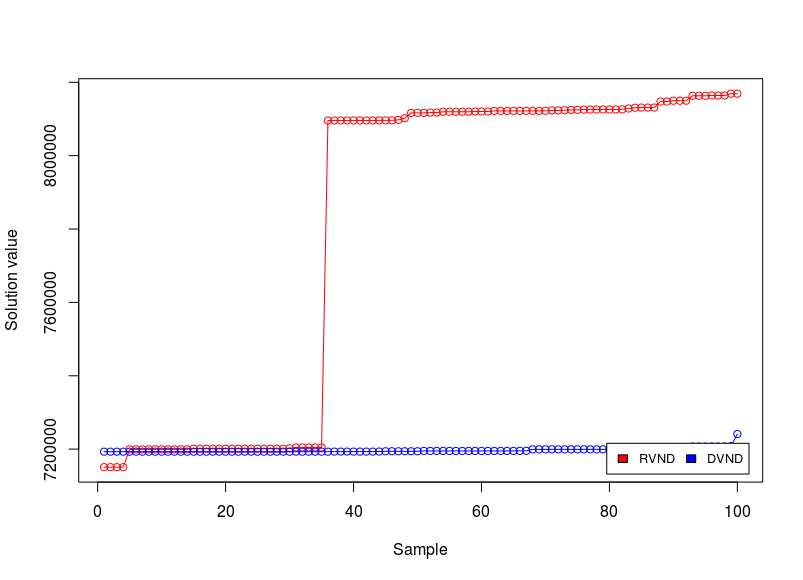
\includegraphics[scale=0.425]{figuras/dvnd/valueDvndRvnd_in2.png}}
% \caption{Valores do DVND e RVND para a instância 2}
% \label{fig:valueDvndRvnd_in2}
% \end{figure}

% Para a instância 3 (veja Figura~\ref{fig:valueDvndRvnd_in3}) RVND obteve melhores resultados para alguns casos e também os piores resultados, contudo em 80 dos 100 testes o DVND obteve melhores resultados.

% \begin{figure}[htbp]
% \centerline{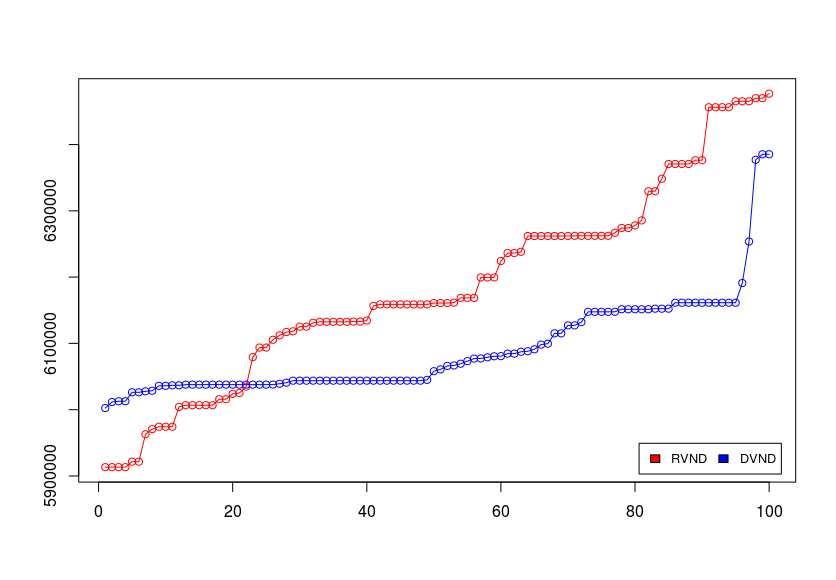
\includegraphics[scale=0.425]{figuras/dvnd/valueDvndRvnd_in3.png}}
% \caption{Valores do DVND e RVND para a instância 3}
% \label{fig:valueDvndRvnd_in3}
% \end{figure}

% Por outro lado, a Figura~\ref{fig:valueDvndRvnd_in4} indica que o RVND obteve melhores resultados para a maioria dos testes da instância 4.
% Contudo novamente o RVND obteve os melhores e também os piores resultados indicando a uma grande variabilidade na qualidade da solução encontrada.

% \begin{figure}[htbp]
% \centerline{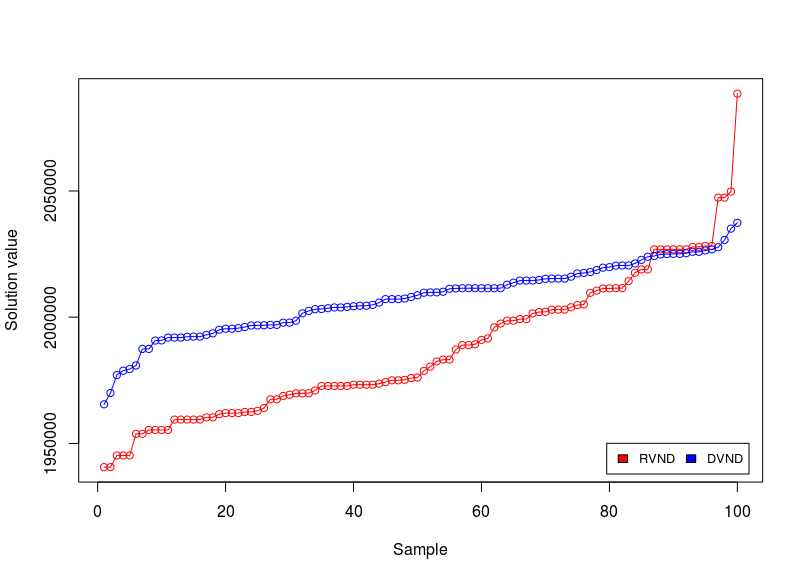
\includegraphics[scale=0.425]{figuras/dvnd/valueDvndRvnd_in4.png}}
% \caption{Valores do DVND e RVND para a instância 4}
% \label{fig:valueDvndRvnd_in4}
% \end{figure}

% \begin{figure}[htbp]
% \centerline{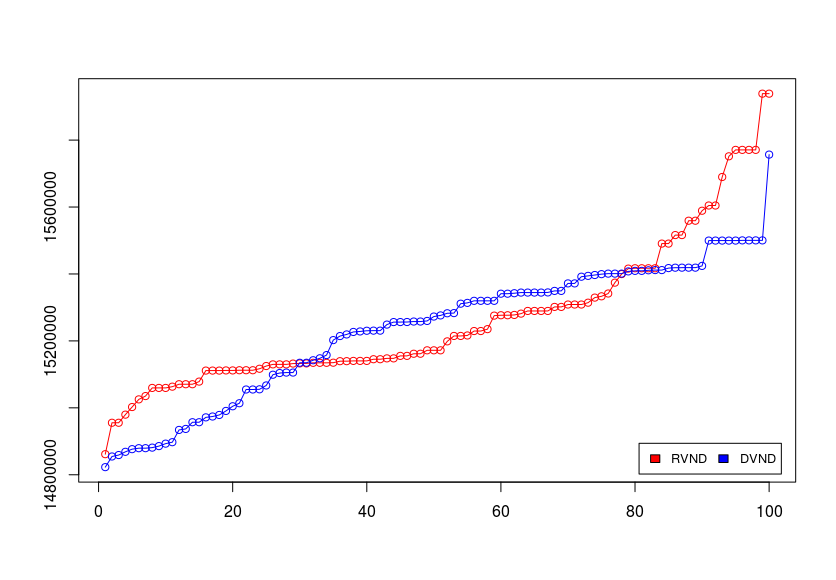
\includegraphics[scale=0.425]{figuras/dvnd/valueDvndRvnd_in5.png}}
% \caption{Valores do DVND e RVND para a instância 5}
% \label{fig:valueDvndRvnd_in5}
% \end{figure}

% Instâncias 5 e 6 (Figura~\ref{fig:valueDvndRvnd_in5}, Figura~\ref{fig:valueDvndRvnd_in6}) obtiveram resultados semelhantes, a última destas manteve uma pequena variação no valor da solução encontrada.

% \begin{figure}[htbp]
% \centerline{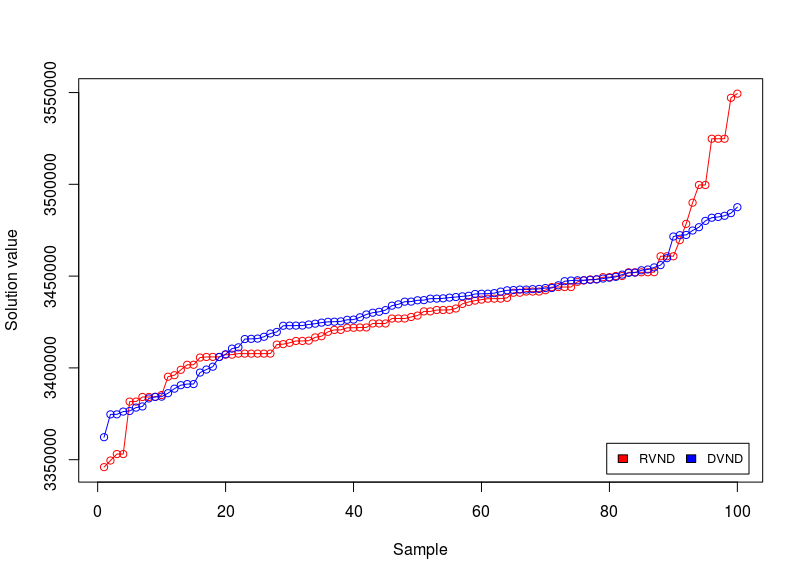
\includegraphics[scale=0.425]{figuras/dvnd/valueDvndRvnd_in6.png}}
% \caption{Valores do DVND e RVND para a instância 6}
% \label{fig:valueDvndRvnd_in6}
% \end{figure}

% A instância 7 tem um comportamento bastante similar ao da instância 4, veja Figura~\ref{fig:valueDvndRvnd_in7} e Figura~\ref{fig:valueDvndRvnd_in4}, o RVND obteve os melhores resultados para alguns testes mas também encontrou os piores valores.

% \begin{figure}[htbp]
% \centerline{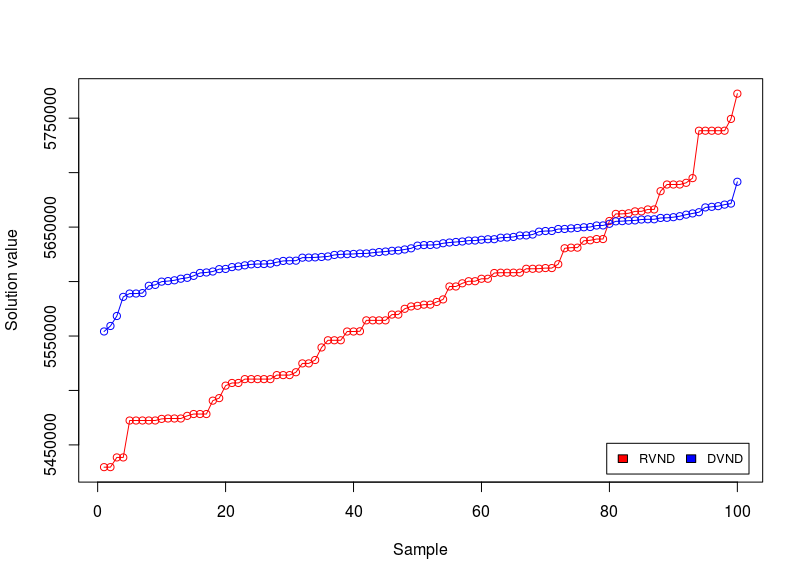
\includegraphics[scale=0.425]{figuras/dvnd/valueDvndRvnd_in7.png}}
% \caption{Valores do DVND e RVND para a instância 7}
% \label{fig:valueDvndRvnd_in7}
% \end{figure}

% Para todas as instâncias os piores resultados das amostragens foram encontrados pelo RVND e este também apresentou uma amplitude maior no valor das soluções, o que pode indicar um forte fator de aleatoriedade na qualidade da solução.
% Desta forma, o objetivo de ter um método de busca local mais profundo e, ao mesmo tempo, mais estável pôde ser alcançado pelo DVND.
% Um outro objetivo era de buscar um algoritmo mais escalável, que pudesse explorar múltiplos nós de processamento simultaneamente, com o objetivo de aproveitar melhor os recursos disponíveis.
